\documentclass{article}
\usepackage{amsmath, amssymb, bm, tikz, mathtools, tcolorbox, array, sfmath, enumerate, multicol, pgfplots}
\renewcommand{\familydefault}{\sfdefault}
\pgfplotsset{compat=newest}
\usetikzlibrary{arrows.meta}
\everymath{\displaystyle}
\tikzset{>=stealth}
\tikzstyle{input} = [circle, text centered, radius = 1cm, draw = black]
\tikzstyle{function} = [rectangle, text centered, minimum width = 2cm, minimum height = 1cm, draw = black]
\usepackage[top = 0.25in, bottom = 0.25in, left = 1in, right = 1in]{geometry}
\pagestyle{empty}
\raggedright

\newcounter{example}[section]
\newenvironment{example}[1][]{\refstepcounter{example}\par\medskip
   {\color{red}\textbf{Example~\theexample. #1}}}{\medskip}

\begin{document}

\section*{Inverse Functions}

\begin{tcolorbox}[colframe=orange!70!white, coltitle=black, title=\textbf{Summary}]
\begin{enumerate}
    \item Inverse functions act as an ``undo" function for a given function.
    \item The graph of the inverse function is a reflection of the original function across $y = x$.
    \item $f^{-1}(\bullet)$ asks you to find the $x$-coordinate associated with the $y$-coordinate of \textbullet.
    % \item The domain of the inverse function is the range of the original.
    % \item The range of the inverse function is the domain of the original.
\end{enumerate}
\end{tcolorbox}
\bigskip 

The {\color{blue}\textbf{inverse}} of the ordered pair $(x,y)$ is $(y,x)$.
\smallskip 

\begin{example}
Find the inverse of each.
\begin{multicols}{2}
\begin{enumerate}[(a)]
    \item $(2,-7)$  
    \item $(0,3)$
\end{enumerate}
\end{multicols}
\end{example}
\vspace{0.25in}

Recall that a function is nothing more than a machine that	
\begin{enumerate}
	\item Accepts an input, $x$		
	\item Performs some operation(s)
	\item Gives an output, $y$
\end{enumerate}
\bigskip 

The inverse function is somewhat of an {\color{blue}\textbf{``undo"}} function.
\newline\\

\begin{center}
\fbox{\parbox{4in}{Inverse functions allow us to take the output of a function, put it into our inverse function, and get our original input value back.}}
\end{center}
\bigskip 

Suppose we put a value of 10 into the function \[f(x) = x^2\]


If we put the output (100) into the inverse, we get our 10 back.	
\bigskip 

\begin{center}
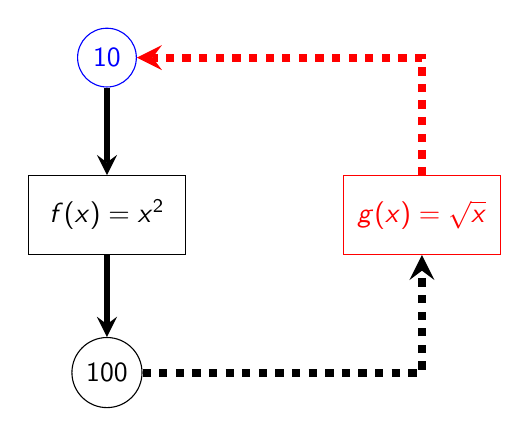
\begin{tikzpicture}[node distance = 2cm]
\node (inputVal) [input, color=blue] {\color{blue}10};
\node (func) [function, below of = inputVal] {$f(x)=x^2$};
\node (outputVal) [input, below of = func] {100};
\node (invFunc) [function, right of = func, xshift = 2cm, color=red] {\color{red}$g(x)=\sqrt{x}$};

\draw [->, >=stealth, thick, line width = 0.75mm] (inputVal) -- (func);
\draw [->, >=stealth, thick, line width = 0.75mm] (func) -- (outputVal);
\draw [->, >=stealth, thick, dashed, line width = 1mm] (outputVal) -| (invFunc);
\draw [->, >=stealth, thick, dashed, line width = 1mm, color = red] (invFunc) |- (inputVal);
\end{tikzpicture}
\end{center}
\vfill 

We use the notation $f^{-1}(x)$ to denote the inverse of $f(x)$.	\newline\\	

\textbf{Note:} The notation {\color{blue}\textbf{does not mean}} raise the function to the $-1$ power.
\vfill 

\textsc{Steps in Finding the Inverse of a Function}
\begin{enumerate}
	\item Rewrite $f(x)=$ as $y=$
	\item Switch your $x$ and $y$ variables.
	\item Solve this result for $y$ and rewrite using inverse notation.
\end{enumerate}
\vfill 
\newpage

\begin{example}
Find the inverse of each of the following.
\begin{enumerate}[(a)]
\begin{multicols}{3}
    \item $f(x) = 5x$
    \item $f(x) = 3x+2$
    \item $f(x) = \dfrac{x+5}{7}$
\end{multicols}
\vfill 
\begin{multicols}{3}
    \item $g(x) = x^3 + 1$
    \item $h(x) = 4x^5 - 1$
    % \item $f(x) = \sqrt{x+3}$   \vfill 
    \item $g(x) = \dfrac{5}{x}$
\end{multicols}
\end{enumerate}
\end{example}

\vfill 
\newpage 

Visually, when finding the inverse of a function, you are {\color{blue}\textbf{reflecting that function across the line $\bm{y = x}$}}.	
\vspace{0.25in}


Below are the graphs of $f(x) = 3x^3-1$ and $f^{-1}(x) = \sqrt[3]{\frac{x+1}{3}}$ as well as the line $y=x$:	\newline\\
\begin{center}
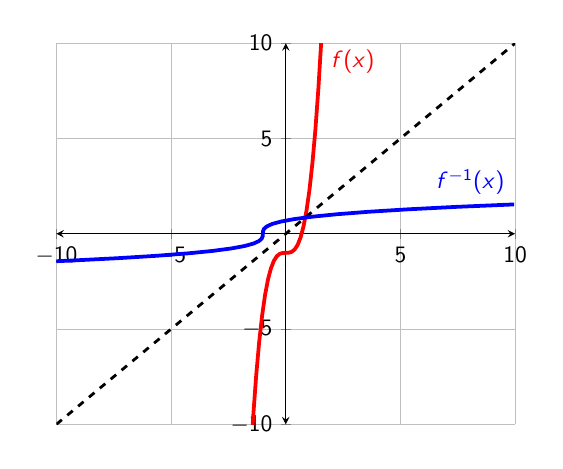
\begin{tikzpicture}[scale=0.85]
\begin{axis}[
	axis lines = middle,
	axis line style=<->,
	grid,
	xmin = -10, xmax = 10,
	ymin = -10, ymax = 10
	]
	\addplot[color=red, ultra thick, domain=-1.55:1.55] {3*x^3-1} node [below right] {$f(x)$};
	\addplot[color=black, very thick, dashed, domain=-10:10] {x};
	\addplot[color=blue, ultra thick, domain=-1.54:1.54] ({3*x^3-1},{x}) node [above left] {$f^{-1}(x)$};
\end{axis}
\end{tikzpicture}
\end{center}
\vspace{0.25in}

%%%%%%%%%%%%%%%%%%%%%%%%%%%

\iffalse

\subsection*{Domain and Range of an Inverse Function}

When switching the $x$ and $y$ in finding the inverse function, you also switch the domain and range of the function and its inverse.		
\vfill 

When you graph a function and its inverse, {\color{blue}\textbf{you'll want to make sure that they are reflections across the line $y=x$}}. This is VERY IMPORTANT for a function such as $y = x^2$.	
\vfill 

This might mean we need to \textbf{restrict the domain and/or range} of our original function.

\[\text{Domain of }f = \text{Range of }f^{-1}\]
\[\text{and}\]
\[\text{Range of }f = \text{Domain of }f^{-1}\]
\vfill 
\newpage

\begin{example}
Find the domain and range of both the function and its inverse.
\begin{enumerate}[(a)]
    \item $f(x) = 5x$   \vfill 
    \item $f(x) = 3x+2$ \vfill 
    \item $g(x) = \sqrt{x+3}$   \vfill \newpage
    \item $f(x) = -\sqrt{x-4}+2$    \vfill 
    \item $f(x) = x^2$ with $x \geq 0$  \vfill 
    \item $f(x) = \dfrac{1}{x}-7$   \vfill \newpage
    \item $f(x)= \dfrac{3}{2x+5}$
\end{enumerate}
\end{example}

\fi 

%%%%%%%%%%%%%%%%%%%%%%%%%%%

\subsection*{Tabular and Visual Approaches to Inverse Functions}

The notation $f^{-1}(\bullet)$ means \underline{what $x$-coordinate has a $y$-coordinate of \textbullet?}
\bigskip 

\begin{example}
Find the value of each.
\begin{center}
\begin{tabular}{c|c|c|c|c|c|c|c|c|c}
    $x$ & $-4$ & $-3$ & $-2$ & $-1$ & 0 & 1 & 2 & 3 & 4 \\ \hline
    $f(x)$ & 2 & 4 & 1 & $-3$ & 0 & 3 & $-4$ & $-1$ & $-2$ \\
\end{tabular}
\end{center}
\vspace{0.25in}
\begin{multicols}{4}
\begin{enumerate}[(a)]
    \item $f^{-1}(3)$
    \item $f^{-1}(-2)$
    \item $f^{-1}(2)$
    \item $f^{-1}(-1)$
\end{enumerate}
\end{multicols}
\end{example}
\vfill 

\begin{example}
Find the value of each given the graph of $f(x)$.
\begin{center}
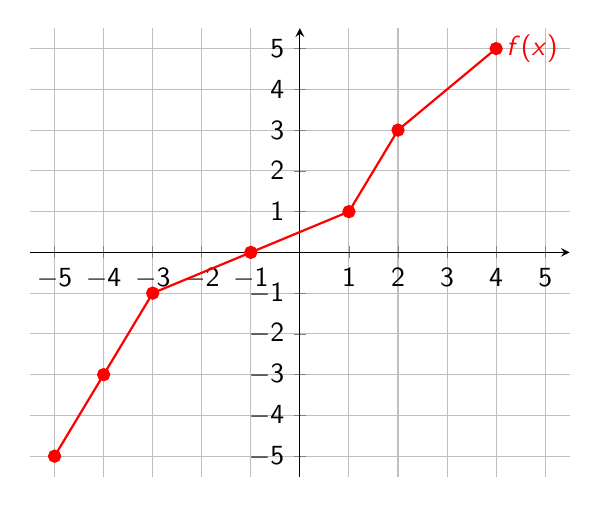
\begin{tikzpicture}
\begin{axis}
    [axis lines = center, xmin = -5.5, xmax = 5.5, xtick = {-5,...,5},
    ymin = -5.5, ymax = 5.5, ytick = {-5,...,5}, grid]
    \addplot[red, mark = *, thick] coordinates {
    (-5, -5) (-4,-3) (-3,-1) (-1,0) (1,1) (2,3) (4,5)
    } node [right] {$f(x)$};
\end{axis}
\end{tikzpicture}
\end{center}
\begin{multicols}{4}
\begin{enumerate}[(a)]
    \item $f^{-1}(-3)$
    \item $f^{-1}(3)$
    \item $f^{-1}(5)$
    \item $f^{-1}(0)$
\end{enumerate}
\end{multicols}
\end{example}
\vfill 

\end{document}
